\chapter{We Are Ecosystems}

\begin{kaichang}
There is probably a cup of yogurt in your refrigerator. Pick it up and read the ingredients: raw milk, white sugar, and a line in small print---Lactobacillus bulgaricus, Streptococcus thermophilus. Notice: these are not preservatives or flavorings, but \textbf{living bacteria}. The manufacturer deliberately puts bacteria into milk; you pay for it, drink it, and feel quite healthy afterward.

Now try something that takes a little more courage: open your mouth and look at your tongue in a mirror. Hundreds of kinds of microorganisms live there right now, numbering in the hundreds of millions. Think a little farther down: your intestines house a microbial world numbering in the trillions. Some people even say that the bacterial cells in your body are about as numerous as your own cells.

First, guess: if you collected and weighed all the bacteria on and inside your body, how much would they weigh? One kilogram? Ten kilograms? Just a small spoonful? At the end of this chapter, we will check your answer---and address a bigger question: are you a ``person,'' or a walking ecosystem?
\end{kaichang}

\section{A Living Universe in a Cup of Yogurt}

First, do what the phenomenon level calls for: describe only what we can see, smell, and measure.

Fresh milk is sweet, with a mild milky aroma; left too long, it spoils and stinks. But introduce the right bacteria at the right temperature, and within a few hours it thickens, turns sour, and becomes yogurt. The sourness comes from lactic acid---bacteria consume the sugar in milk and release lactic acid, which makes the milk proteins coagulate (acid denaturation of proteins was discussed in Chapter 47). Every sour mouthful and every bit of thickness you experience come from bacterial metabolic ``waste'' and its by-products.

Now consider your body. Your skin feels clean, but under a microscope it resembles rolling plains, with staphylococci and propionibacteria living in the valleys. Your warm, moist mouth is a ``tropical rainforest'' for hundreds of bacterial species. Your large intestine---dark, warm, oxygen-poor, and supplied with a constant stream of food residues---is the body's busiest microbial metropolis.

They actually leave plenty of ``observable traces''; you simply may not have thought of them that way. Morning breath is the smell of products left by oral bacteria breaking down food residues overnight. Sweat itself has almost no odor; armpit odor comes from small molecules released when skin bacteria break down its ingredients. That soft deposit scraped off your toothbrush as you brush---dental plaque---is a genuine ``bacterial community,'' with dozens or hundreds of species settling in layers, like a three-dimensional city.

Most of the time, though, you really cannot feel them. No itching, no sound. Only in the last twenty or thirty years did scientists truly count the scale of this world. They stopped relying on the old method of ``grow the bacteria, then count them'' (many gut bacteria cannot be grown outside the intestine), and instead used DNA sequencing to ``take attendance'': read microbial gene fragments directly from a sample, then match them to identify who is there.

\section{Counting Your Microbial Tenants}

Here is the first part of the answer to our opening puzzle. Scientists estimate that an ordinary adult's intestines contain about $3.8\times 10^{13}$ bacterial cells---thirty-eight trillion. Your own human cells number about $3\times 10^{13}$. The two counts have the same order of magnitude; bacteria even have a slight lead.

Before you gasp, an honest qualification: bacterial cells are much smaller than human cells. An E. coli cell has roughly one-thousandth the volume of an ordinary human cell. So by \textbf{weight}, these microbes together amount to only about $0.2$ kilograms---a small bag of salt, not several kilograms. Did you guess correctly?

\begin{qiaoliang}
How is this estimate made? You can reproduce the reasoning. Scientists measure about $10^{11}$ bacterial cells per gram of feces, then estimate that the large intestine contains a few hundred grams of material. Multiplication gives the total gut bacterial population (bacteria elsewhere in the body are negligible by comparison). The same kind of estimate works for yogurt: live-culture yogurt that meets standards contains roughly $10^{8}$ or more living bacteria per milliliter. Drink a $150$-milliliter cup, and you swallow tens of billions of live bacteria in one gulp---more than the world's human population. Think of that number next time you drink yogurt.
\end{qiaoliang}

Their number is not the most astonishing part. Their \textbf{variety} is: your gut contains roughly hundreds to over a thousand different microbial species, carrying a total number of genes over a hundred times the number in your own genome. Genetically speaking, most of the books in the library called ``you'' are not written in your own script. Remember that detail: at the chapter's end, it becomes a doorway into Volume III.

\section{From Tenants to an Ecosystem}

Zoom in to the particle level---this chapter's ``particles'' are individual microbial cells and the molecules flowing between them.

Chapter 57 explained that a cell is a chemical city capable of maintaining itself. What happens when trillions of cells crowd into your gut? What happens in any crowded world: competition for resources, territorial claims, cooperation, and mutual exploitation. In other words, \textbf{ecology}.

Ecologists studying a forest distinguish relationships between species. Move their vocabulary into your belly, and almost nothing needs changing:

\begin{itemize}[itemsep=2pt]
\item \textbf{Mutualism}: You eat dietary fiber you cannot digest; gut bacteria ferment it for you, and the resulting short-chain fatty acids nourish your intestinal lining. You provide the accommodation (food and shelter); they pay rent (nutrition and protection).
\item \textbf{Commensalism}: Many skin bacteria live on you, eating oils and dead skin without obviously helping or harming you---just tenants living rent-free.
\item \textbf{Competition}: With the same territory and nutrients, whoever gets there first claims them. Dense native populations fill the gut's ecological niches, often leaving harmful newcomers no room. A healthy microbial community is itself a defense, a ``civilian police force'' beyond the immune defenses of Chapter 61.
\item \textbf{Parasitism and disease}: A few tenants turn hostile. Helicobacter pylori drills holes in the stomach; Candida albicans multiplies excessively when your defenses weaken. The same microorganism may be a quiet lodger under ordinary conditions and a troublesome tenant when conditions change---this is ``opportunistic infection.''
\end{itemize}

Your gut world therefore follows the same kinds of rules as a forest or coral reef: abundance depends on food, space, acidity, and who competes or cooperates with whom. Your body is not a pristine fortress ``invaded'' by bacteria. It has been an ecosystem from the beginning---one in which you and microorganisms have coevolved for hundreds of millions of years.

\section{The Gut: A Fermentation Factory}

The most important rules in an ecosystem govern the flow of matter and energy. Consider your gut's ``industrial structure.''

Your small intestine handles digestion and absorption: enzymes break starch into glucose (Chapter 46), proteins into amino acids, and fats into fatty acids---all familiar from Chapter 55's metabolic network. But your enzymes cannot break down one class of food: dietary fiber, including certain complex carbohydrates in beans, whole grains, and vegetables. These pass through the small intestine unchanged into the large intestine.

Your enzymes cannot do the job, but that does not mean no enzymes can. Gut bacteria have a chemical toolkit you lack. They ferment these fibers into small molecules called \textbf{short-chain fatty acids}: acetic acid, propionic acid, and butyric acid. Do not underestimate this ``bacterial exhaust'': butyrate is the main food for cells lining your large intestine; acetate and propionate enter the blood and participate in energy metabolism and signaling throughout the body (Chapter 58 explained how cells receive messages---bacterial products are messages too).

Write this in symbols. Lactic acid fermentation in yogurt is the bacterial version of glycolysis (Chapter 49): one glucose molecule is split, yielding a net two ATP, while the remaining skeleton becomes lactic acid---
\[\chem{C_6H_{12}O_6} \rightarrow 2\,\chem{C_3H_6O_3}\]
Notice that the numbers of atoms balance on both sides. This is the conservation of mass from Chapter 26: bacteria have not ``destroyed'' sugar, but extracted a small part of its energy and excreted its remaining skeleton in a different form. The sourness you taste is the product on the right.

Gut fermentation produces other ``by-products.'' One class is gases: hydrogen, carbon dioxide, and, in some people's microbial communities, methane. These are the main sources of intestinal gas; most of what you pass each day is not ``swallowed air,'' but emissions from bacterial fermentation chimneys. Another class is vitamins: some gut bacteria synthesize vitamin K and several B vitamins, some of which the body can absorb and use. Your ``tenants'' pay part of their own food bill.

\begin{center}
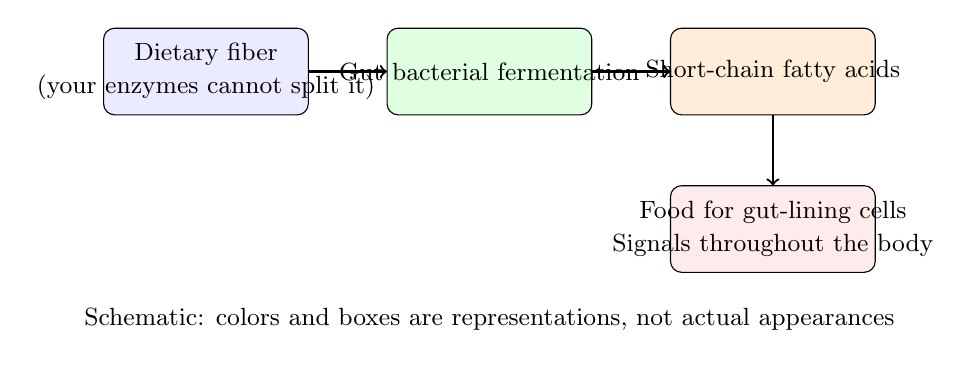
\begin{tikzpicture}[scale=1]
\draw[rounded corners, fill=blue!8] (0,0) rectangle (2.6,1.1);
\node[align=center] at (1.3,0.55) {\small Dietary fiber\\ \small (your enzymes cannot split it)};
\draw[->, thick] (2.6,0.55) -- (3.6,0.55);
\draw[rounded corners, fill=green!12] (3.6,0) rectangle (6.2,1.1);
\node[align=center] at (4.9,0.55) {\small Gut bacterial fermentation};
\draw[->, thick] (6.2,0.55) -- (7.2,0.55);
\draw[rounded corners, fill=orange!15] (7.2,0) rectangle (9.8,1.1);
\node[align=center] at (8.5,0.55) {\small Short-chain fatty acids};
\draw[->, thick] (8.5,0) -- (8.5,-0.9);
\draw[rounded corners, fill=red!8] (7.2,-2.0) rectangle (9.8,-0.9);
\node[align=center] at (8.5,-1.45) {\small Food for gut-lining cells\\ \small Signals throughout the body};
\node[align=center] at (4.9,-2.6) {\small Schematic: colors and boxes are representations, not actual appearances};
\end{tikzpicture}
\end{center}

\begin{shiyan}
\textbf{Make yogurt at home and see bacteria at work.}

Materials: $500$ milliliters of plain milk (pasteurized or shelf-stable), two spoonfuls of commercial plain live-culture yogurt (look for ``live cultures'' in the ingredients), a clean glass jar, and plastic wrap.

Steps: (1) Scald the glass jar with boiling water and let it dry. (2) Warm the milk to about $40\,^{\circ}\mathrm{C}$ (warm, not hot, to the touch), then stir in two spoonfuls of yogurt. (3) Pour into the jar and cover; wrap in a towel and leave undisturbed somewhere warm (about $35$--$40\,^{\circ}\mathrm{C}$) for $6$--$10$ hours. (4) Refrigerate once set.

Observations: Check every two hours and record the change from liquid to semisolid. Smell how the sourness changes. Think: why must you add a ``starter culture''? Why would simply leaving milk somewhere warm only make it spoil?

Safety: Use clean utensils throughout; refrigerate the finished yogurt and eat it within a day or two. If it smells rotten or shows mold, discard the whole jar without tasting it. Do not use raw milk.
\end{shiyan}

\textbf{Translator safety note:} The source recipe is not a complete food-safety protocol: touch does not measure temperature, and a towel does not control incubation. For yogurt intended for eating, follow a tested procedure with a thermometer, its specified heating and incubation temperatures, and prompt refrigeration; see \href{https://extension.oregonstate.edu/sites/default/files/documents/8836/fs173emakingyogurt.pdf}{university Extension yogurt guidance}. An adult should handle hot milk, water, and glass. Do not taste a classroom culture or rely on its smell to establish safety.

\section{A Culture Tube Overturns a Medical Consensus}

\begin{zhengju}
The most famous ``villain'' in your microbial world is probably Helicobacter pylori. It lives in the stomach and is associated with gastritis, stomach ulcers, and stomach cancer. Before 1982, however, medicine spoke almost with one voice: the stomach contains strong acid (its pH can fall to 1.5), so no bacteria can live there long-term; ulcers result from stress, spicy food, and excess acid secretion. Doctors prescribed stress reduction, liquid diets, acid-suppressing drugs, and, in severe cases, surgical removal of part of the stomach.

In 1979, Australian pathologist Warren repeatedly saw small curved bacteria in stomach-lining sections from patients with gastritis. Wherever these bacteria appeared, the lining was almost always inflamed. His colleague, the young physician Marshall, took the matter seriously: he cultured the bacteria from patients' stomachs and searched the literature, discovering that the claim ``the stomach is sterile'' itself lacked solid evidence.

What followed sounds legendary, but notice how it follows each step of the scientific method. Marshall first tried animal experiments with the cultured bacteria, without successfully causing disease. In 1984, he performed an experiment that no ethics committee today would approve: he personally drank a tube of H. pylori culture. Days later, he developed nausea and vomiting, and endoscopy confirmed acute gastritis. Bacteria first, inflammation afterward: the time sequence fit. More decisive evidence followed: after antibiotics killed these bacteria, many patients with stubborn ulcers recovered, and recurrence fell sharply. If ulcers really were ``caused by stress,'' why would antibiotics cure them?

Alternative explanations were eliminated one by one, forcing the consensus to change. Warren and Marshall received the Nobel Prize in 2005. The story has a thought-provoking postscript: H. pylori has lived alongside humans for at least tens of thousands of years, and scientists now find that it may have another, more ``tenant-like'' side (for example, an association with a lower incidence of gastroesophageal reflux disease). The boundary between ``villain'' and ``resident'' is blurrier than anyone then imagined. In an ecosystem, there are no absolutely good or bad microbes, only members playing particular roles under particular conditions.
\end{zhengju}

\textbf{Translator safety note:} Marshall's self-experiment is history, not an activity to imitate: do not grow or ingest pathogens. The possible association described above is not a reason to retain an infection or stop treatment. H. pylori can cause ulcers and requires clinician-directed diagnosis and treatment; see \href{https://www.niddk.nih.gov/health-information/digestive-diseases/peptic-ulcers-stomach-ulcers/treatment}{NIDDK ulcer-treatment guidance}.

\section{Antibiotics: Selection on Fast-Forward}

After Fleming discovered penicillin in 1928, humans for the first time held a weapon for ``precision bombing'' bacteria. Antibiotics work chemically: they target structures or machinery unique to bacteria, for example by inhibiting cell-wall synthesis or jamming bacterial ribosomes. Human cells lack these components, so the drugs can kill bacteria relatively selectively.

But notice ``relatively.'' Once inside the body, antibiotics cannot distinguish the gut's ``good lodgers'' from its ``bad tenants.'' A course of broad-spectrum antibiotics can flatten whole neighborhoods of the gut community. Recovery may take months, and some members may never return. This is why doctors insist that antibiotics be used for the prescribed course and the appropriate indications: do not take them casually yourself, or stop on your own after two days because you feel better.

A more serious problem follows. Suppose a tiny minority in a bacterial population happen, through random genetic differences, to be less vulnerable to an antibiotic. The drug arrives and sensitive bacteria die en masse. The lucky survivors suddenly have abundant vacant space and food; they multiply rapidly, and the next generation's entire population withstands the drug. This is \textbf{antibiotic resistance}: essentially a live broadcast of natural selection compressed into weeks.

One point must be absolutely clear: bacteria do \textbf{not} ``encounter a drug and then work hard to learn to resist it.'' Variation arises randomly before exposure; the drug is merely a ``selector,'' leaving behind individuals that happen to resist it. Individuals do not change because they need to; the proportions of types in the population change. We will repeatedly return to this rule in Volume III's discussion of evolution. Today, antibiotic misuse (including in livestock farming) is selecting ever more bacteria into ``superbugs,'' considered one of the major threats to global public health.

Antibiotics reveal the ecosystem's nature in another way. Clostridium difficile is among the few gut bacteria capable of forming resistant spores. Normally, dense native populations keep it suppressed. After broad-spectrum antibiotics remove many natives, it may bloom, causing severe and even life-threatening diarrhea. This is not ``a stronger enemy invading,'' but ``an inconspicuous local thug taking over the neighborhood after the police are defeated.'' Remarkably, one of the most effective treatments is to transplant a healthy donor's gut community back in, letting a complete ecosystem restore order. Treatment shifts from ``kill bacteria'' to ``restore ecology'': a profound change in medical thinking.

\textbf{Translator safety note:} Fecal microbiota treatment is not a do-it-yourself remedy. Even material from screened donors can transmit dangerous pathogens; treatment requires specialist assessment and appropriate safeguards. See the \href{https://www.fda.gov/safety/medical-product-safety-information/fecal-microbiota-transplantation-safety-alert-risk-serious-adverse-events-likely-due-transmission}{FDA safety alert}. Seek medical advice for severe or persistent diarrhea, especially after antibiotics.

\section{Communities Change: Diet, Age, Drugs, Environment}

An ecosystem never stands still. Your microbial community changes daily with your life:

\begin{itemize}[itemsep=2pt]
\item \textbf{Diet}: Several days of eating lots of meat versus lots of whole grains and beans produce noticeably different dominant gut communities. Fiber-fermenting bacteria thrive on ``high-fiber meals.'' Long-term dietary patterns have a still larger effect.
\item \textbf{Age}: Babies acquire their first microbial ``seeds'' through the birth canal and breast milk; it takes years for the community to become adult-like. In older people, diversity usually declines again.
\item \textbf{Medicines}: Antibiotics act most directly. Some common medicines, such as acid suppressants, also change the gut environment, indirectly changing who can survive there.
\item \textbf{Environment}: The people you live with, household pets, and the soil and water you touch all exchange microbes with you. Family members under one roof often have more similar communities than strangers do.
\end{itemize}

You may now wonder: if microbial communities matter so much, can adjusting them treat disease, reduce weight, or improve mood? This is among the hottest fields of the past decade or so, and among those most in need of clear heads. Let us discuss it at the boundary level.

\section{Boundaries: The Model's Power and Limits}

The ``human as ecosystem'' model is very useful: it explains why antibiotics can cause diarrhea, why dietary fiber benefits health, and why incoming pathogens sometimes struggle to establish themselves. But it has clear boundaries. This chapter also encounters some of science communication's most widespread exaggerations, which must be addressed individually.

\textbf{First, correlation is not causation.} Many studies find that the gut communities of people with obesity, diabetes, or depression are ``different'' from those of healthy people. Difference does not establish that microbes are the cause: disease or diet may change the community, or causation may run both ways. Moving from ``associated with'' to ``causes'' requires experimental evidence like Marshall's: change the community, see whether the outcome changes, and exclude other explanations.

\textbf{Second, claims that ``one bacterium determines personality'' lack sufficient evidence at present.} You may have seen short videos or advertisements saying ``the gut is your second brain; this bacterium makes you outgoing'' or ``take this probiotic to become smarter.'' The actual research picture is this: germ-free mice do show behavioral effects when microbes are absent, and a few small human studies report associations between microbial communities and mood. But mice are not people; small studies often cannot be replicated; and human personality reflects genes, upbringing, social experience, and more. Between ``microbes are associated with mood'' and ``one bacterium determines your personality'' lies an entire unfinished chain of evidence. A sound response is: interesting, awaiting verification, keep your wallet closed for now.

\textbf{Third, microbiome research is still young.} Different laboratories analyzing the same person's microbes may obtain different results because their methods differ. Many conclusions describe statistical averages that cannot be applied to a particular individual. Only a handful of microbial interventions have firmly established medical value. Fecal microbiota transplantation for recurrent C. difficile infection is the most successful example, supported by randomized controlled trials, but it has strict indications and procedures. It is certainly not evidence that ``changing your microbes cures everything.''

\section*{Common Misconceptions}

\begin{wuqu}
``Probiotics are health supplements; more cannot hurt. A probiotic drink is all you need to improve your constitution.'' This misconception has two layers. First, after passing the ``checkpoints'' of stomach acid and bile, few organisms in most probiotic products can settle long-term in your gut; most are merely ``passing visitors.'' For healthy people, claimed benefits often lack high-quality trial evidence. The subtler second layer treats the gut community as a simple pond where you ``add whatever is missing,'' ignoring an ecosystem of a thousand competing and cooperating species. One or two newcomers rarely transform the whole community. Instead of paying for bacteria, feed those you already have: varied vegetables, fruit, and whole grains are the most tangible ``subsidy'' for your gut ecosystem. (If you actually need treatment for an illness, listen to your doctor, not advertisements.)
\end{wuqu}

\section{Back to That Cup of Yogurt}

Return to our opening cup. You can now reread its ingredients ecologically: L. bulgaricus and S. thermophilus are two tenants ``selected'' by humans to cooperate in the temporary ecosystem of milk. One breaks down some protein first, helping the other grow. They work in relay to turn lactose into lactic acid, until conditions become too acidic even for themselves and fermentation stops. You think you are drinking milk; actually, you are receiving a miniature ecosystem's metabolic legacy.

Most of the bacteria you swallow are only passing through. They must cross the strong-acid checkpoint of the stomach (the protein-denaturing environment discussed in Chapter 52) and pass through bile; very few finally reach the large intestine alive. Even those that arrive struggle to settle in niches already packed with native residents. This does not mean yogurt is bad---it is a good food---but that your $0.2$-kilogram ecosystem of thirty-eight trillion tenants has a stubborn inertia of its own.

And the bigger question: are you a person or an ecosystem? The answer is that you have never been ``purely human.'' Your mitochondria are bacteria that moved in over a billion years ago (Chapter 57's evidence for endosymbiosis); your gut is a metropolis of a thousand species; your skin is another continent. Under biology's magnifying glass, the boundaries of ``I'' are blurry.

\section{Volume II Ends; Information Begins}

Volume I of this book went from fundamental particles to chemical reactions; Volume II has taken us from carbon atoms to here. Carbon builds organic molecules, organic molecules form macromolecules, macromolecules assemble into cells, cells gather into bodies, and bodies join microorganisms in ecosystems. Matter's chain links together without a single link requiring a miracle.

But perhaps you noticed a question we repeatedly sidestepped: \textbf{information}. Why can bacteria ferment lactose? Because they carry genes encoding lactase. Why are resistant bacteria's offspring born resistant? Because the ``spelling'' of resistance was copied. Why do you resemble your parents more than your deskmate? Why is your microbial community more like your family's?

``Structure'' and ``energy'' can no longer answer these questions. They point to another thread: what symbols does life use to record recipes, how does it copy those records, and what happens when copying goes wrong? Your thirty-eight trillion microbial tenants copy their records every time they divide, while every cell in your body contains an instruction manual written in three billion letters. Volume III starts here: Chapter 63 returns to a nineteenth-century monastery garden to see how Mendel used peas to turn ``heredity'' from mysticism into arithmetic. Then we will follow the trail to DNA's double helix and today's technologies for rewriting genes.

\begin{tiaozhan}
How do ecologists assign a number to ``community diversity''? One common tool is the Shannon diversity index: $H=-\sum p_i \ln p_i$, where $p_i$ is the fraction of the community belonging to species $i$. Try calculating it: community A has two species, each making up half; community B also has two species, in a $99:1$ ratio. A has $H\approx 0.69$, B has $H\approx 0.06$. The same two species, but different evenness makes an enormous difference in diversity. A healthy gut community resembles A: diverse and structurally stable. After antibiotic misuse, it may slide toward B, dominated by one or two species. Researchers often use falling diversity as a rough signal of ``ecological imbalance,'' but remember this chapter's boundaries: the relationship between diversity and health is also statistical, not an individual diagnosis. You can skip this section without losing the main thread.
\end{tiaozhan}

\section*{Try It Yourself}

\begin{sikaoti}
\item Draw a material-flow diagram of ``your day'': where are breakfast starch, dietary fiber, and protein processed, by whom (your enzymes or gut microbes), and where do the products go? Mark with arrows the part ``bacteria do for you because you cannot.''
\item An E. coli cell weighs about $10^{-12}$ grams. If a person's gut contains about $4\times 10^{13}$ bacteria, estimate their total mass and compare it with the text's ``about $0.2$ kilograms.'' What uncertainties enter this estimate?
\item Explain to your deskmate in your own words why ``bacteria encounter antibiotics and work hard to learn resistance'' is wrong. Draw the community at three times---before treatment, after treatment, and after reproduction---using dots for sensitive bacteria and triangles for resistant ones.
\item You see a report titled ``Scientists Discover: This Gut Bacterium Makes People More Outgoing.'' What three questions would you ask to assess its reliability? (Hint: consider the sample, causation, and reproducibility.)
\item Why did ``stomach acid is strong, so there are no bacteria in the stomach'' once sound reasonable, yet turn out to be wrong? What does this story teach about why apparently reasonable ``mechanistic inferences'' still need experimental testing?
\end{sikaoti}
